\documentclass{article}
\usepackage{fullpage}
\usepackage{multicol,multirow}
\usepackage{tabularx}
\usepackage{ulem}
\usepackage[utf8]{inputenc}
\usepackage[russian]{babel}
\usepackage{pgfplots}
\usepackage{graphicx}

\begin{document}

\section*{Лабораторная работа №7 по курсу «Численные методы»}

Выполнил студент группы М8О-408Б-20 Блинов Максим.
\\
Преподаватель: Пивоваров Д.\,Е.

\subsection*{Цель}

Решить краевую задачу для дифференциального уравнения эллиптического типа. 
Аппроксимацию уравнения произвести с использованием центрально-разностной схемы. 
Для решения дискретного аналога применить следующие методы: метод простых итераций (метод Либмана), 
метод Зейделя, метод простых итераций с верхней релаксацией. Вычислить погрешность численного решения 
путем сравнения результатов с приведенным в задании аналитическим решением . Исследовать зависимость 
погрешности от сеточных параметров .

\subsection*{Вариант 3}
$$
\frac{\partial^2 u}{\partial x^2} + \frac{\partial^2 u}{\partial y^2} = 0,
$$

$$
u(0, y) = \cos y,
$$

$$
u(1, y) = e \cos y,
$$

$$
u_y(x, 0) = 0,
$$

$$
u_y\left(x, \frac{\pi}{2}\right) = -\exp(x).
$$

Аналитическое решение:
$$
U(x, y) = \exp(x) \cos y.
$$




\subsection*{О программе}

Программа была реализована на языке программирования Go и включает в себя три численных метода для решения дифференциальных уравнений: 
метод Либмана, метод Зейделя и метод простых итераций с верхней релаксацией. Для визуализации результатов использовалась библиотека Gonum, 
которая предоставляет широкие возможности для построения графиков в среде Go. Результаты вычислений иллюстрируют поведение решений в зависимости от времени 
и начальных условий, а также позволяют оценить точность численных методов путём сравнения с аналитическим решением задачи. 
Графики ошибок демонстрируют различия между аналитическими и численными решениями на протяжении всего временного интервала. 
Все вычислительные эксперименты и генерация графиков проводились в рамках данной программы.

\subsection*{Инструкция к запуску}
Для запуска программы на Go, решающей гиперболические дифференциальные уравнения, убедитесь, что у вас установлена последняя версия Go 
(на данный момент 1.21, проверьте на официальном сайте). Создайте рабочее пространство, затем установите необходимые зависимости go mod tidy.

\pagebreak

\subsection*{Метод Либмана}

Метод Либмана, также известный как метод Гаусса — Зейделя или метод последовательных замещений, является итерационным методом для решения систем 
линейных уравнений. Он работает путем последовательного приближения к решению, используя предыдущие оценки для вычисления текущей. Этот метод особенно 
полезен, когда решается большая система уравнений, так как может быть более эффективным по сравнению с другими методами, такими как прямое решение.
\\
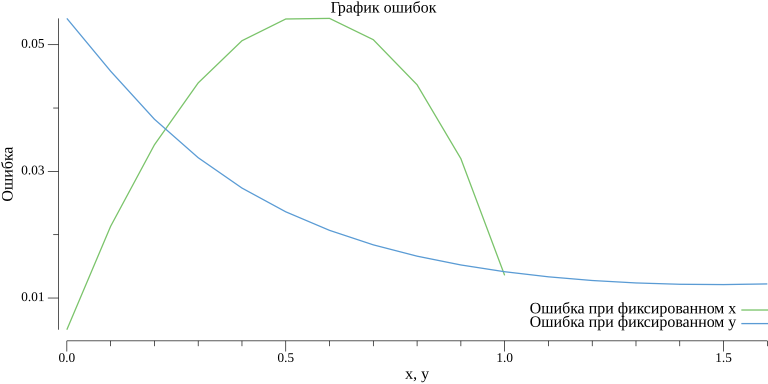
\includegraphics[scale=0.6]{error_plot_0.png}
\\

\\
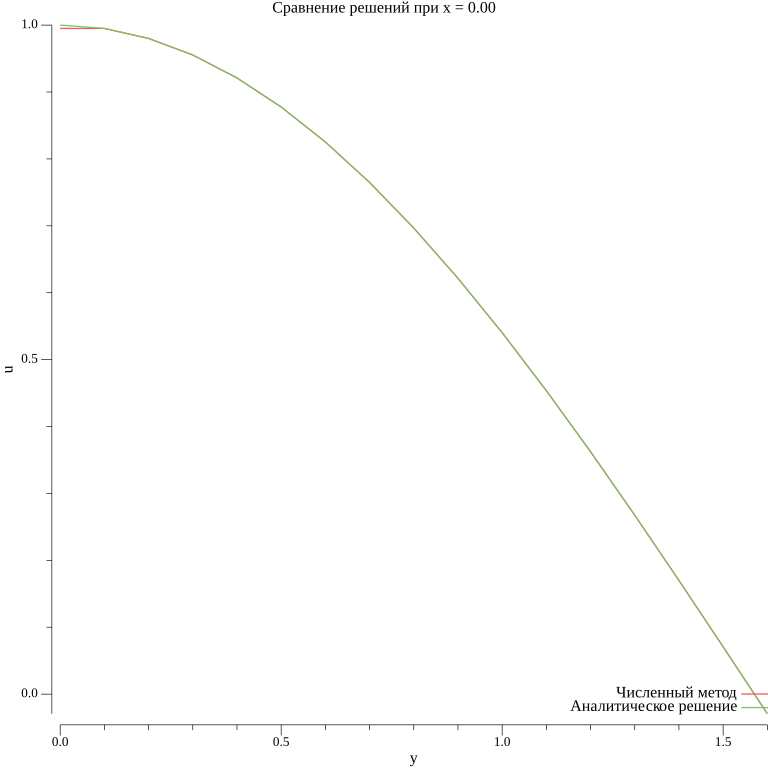
\includegraphics[scale=0.6]{0plot_x_0.00.png}
\\

\\
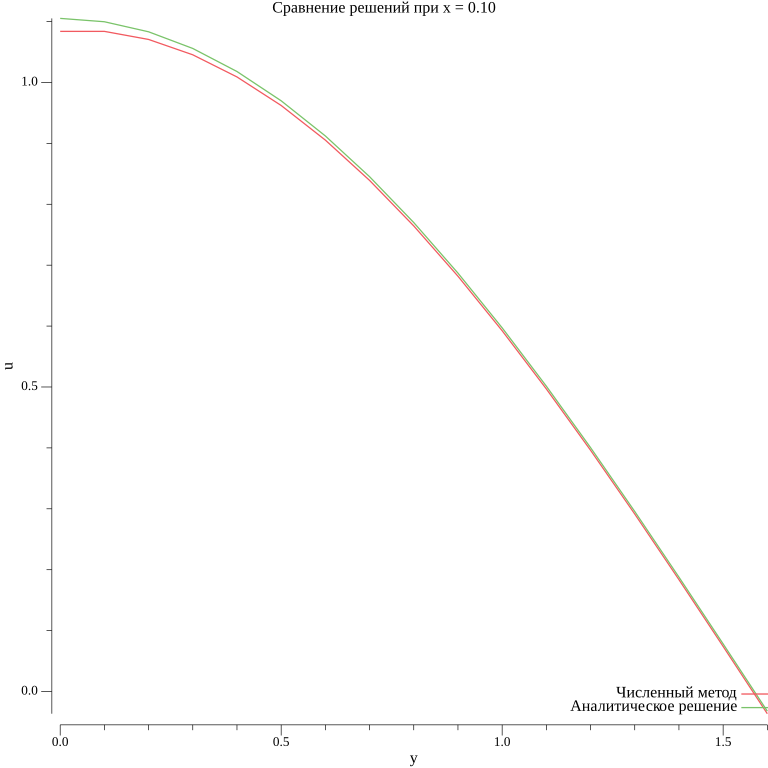
\includegraphics[scale=0.6]{0plot_x_0.10.png}
\\

\\
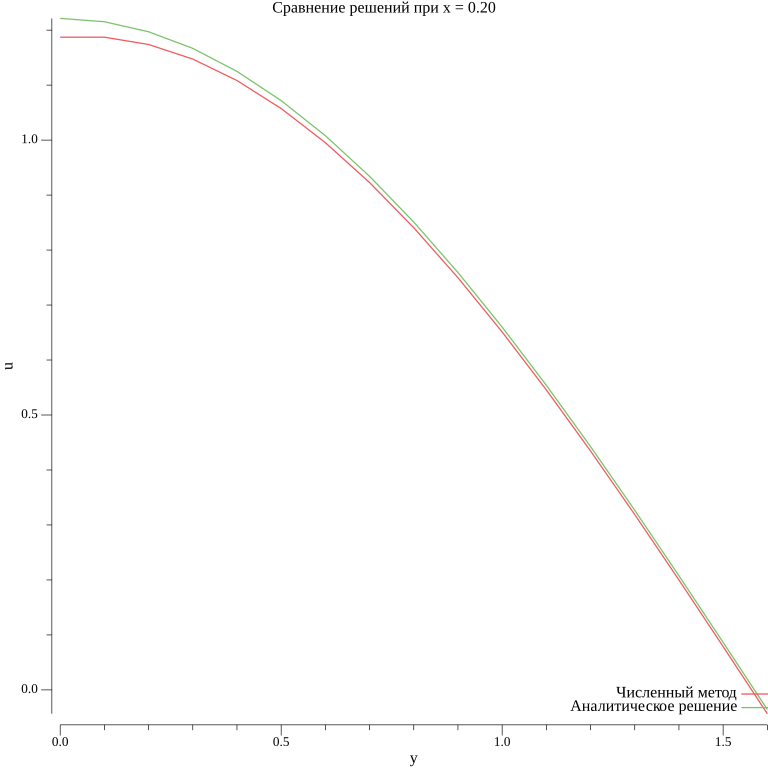
\includegraphics[scale=0.6]{0plot_x_0.20.png}
\\

\\
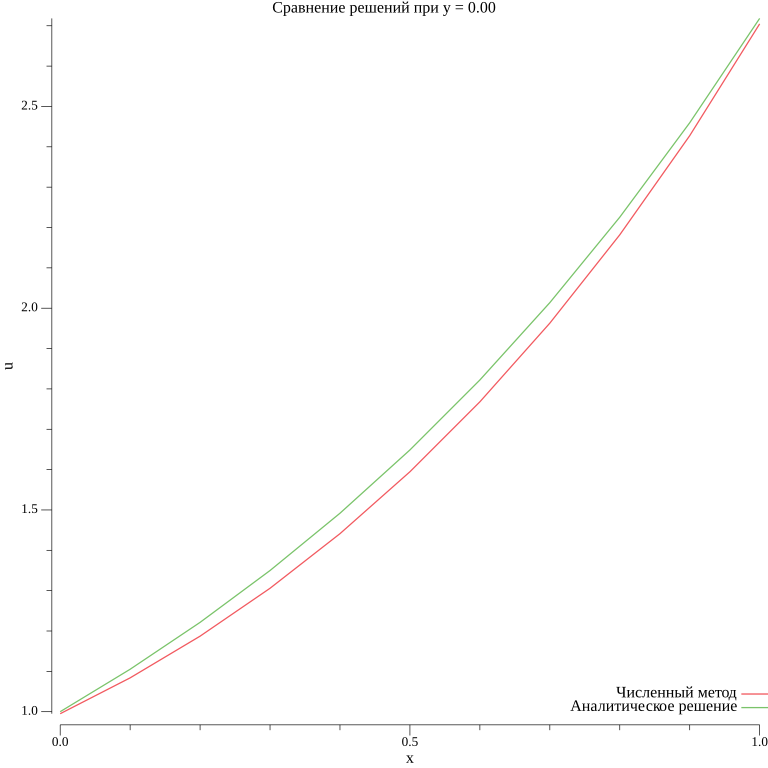
\includegraphics[scale=0.6]{0plot_y_0.00.png}
\\

\\
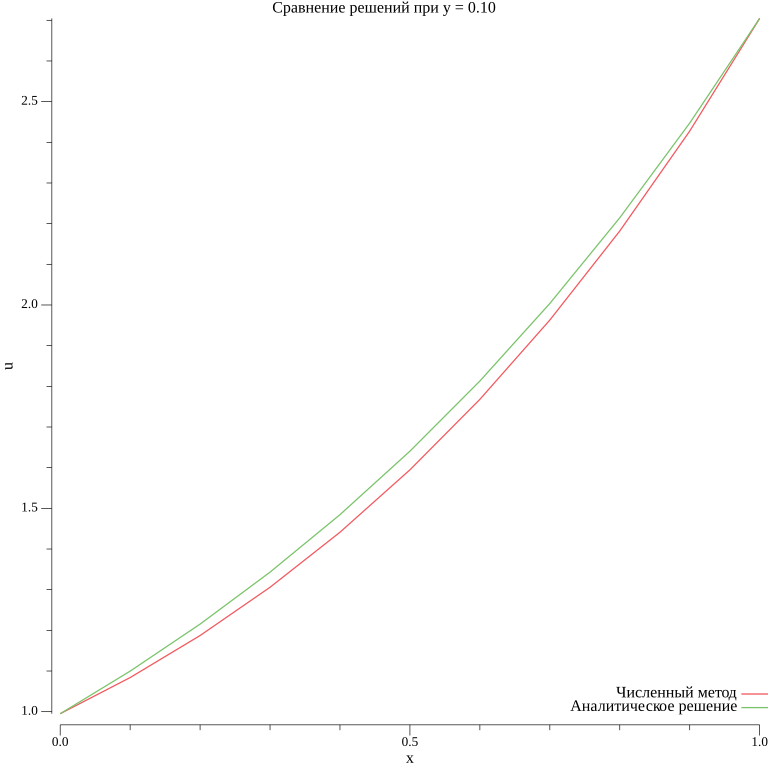
\includegraphics[scale=0.6]{0plot_y_0.10.png}
\\

\\
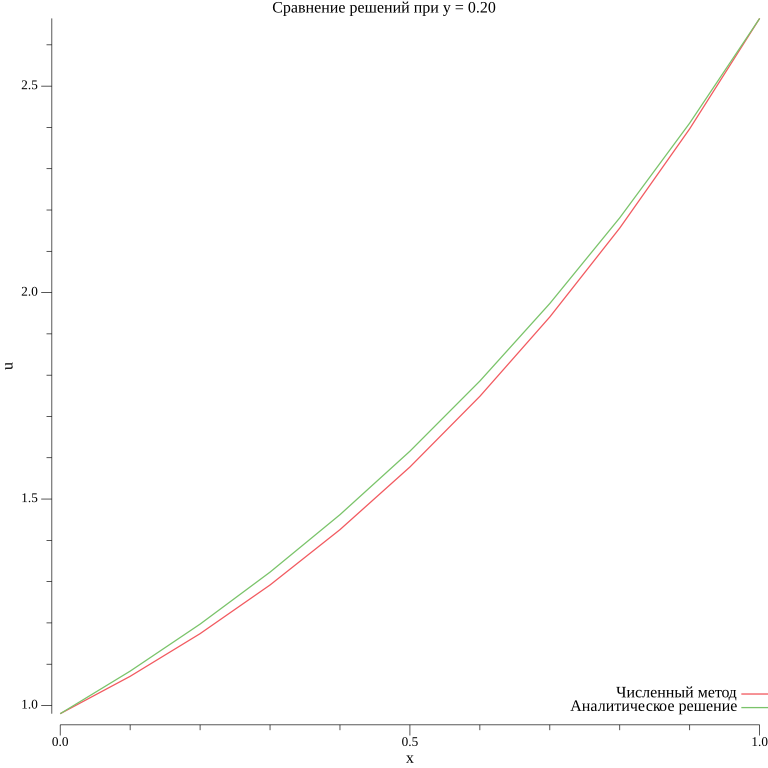
\includegraphics[scale=0.6]{0plot_y_0.20.png}
\\

\subsection*{Метод Зейделя}
\\
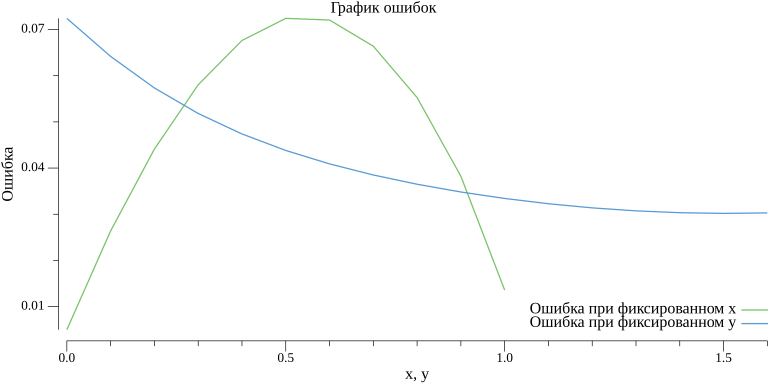
\includegraphics[scale=0.6]{error_plot_1.png}
\\

\\
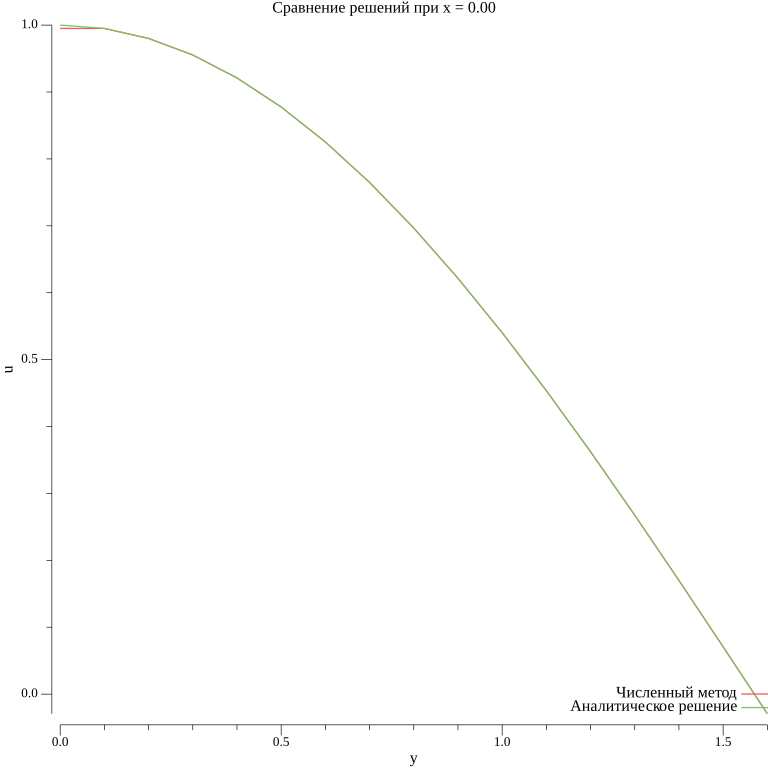
\includegraphics[scale=0.6]{1plot_x_0.00.png}
\\

\\
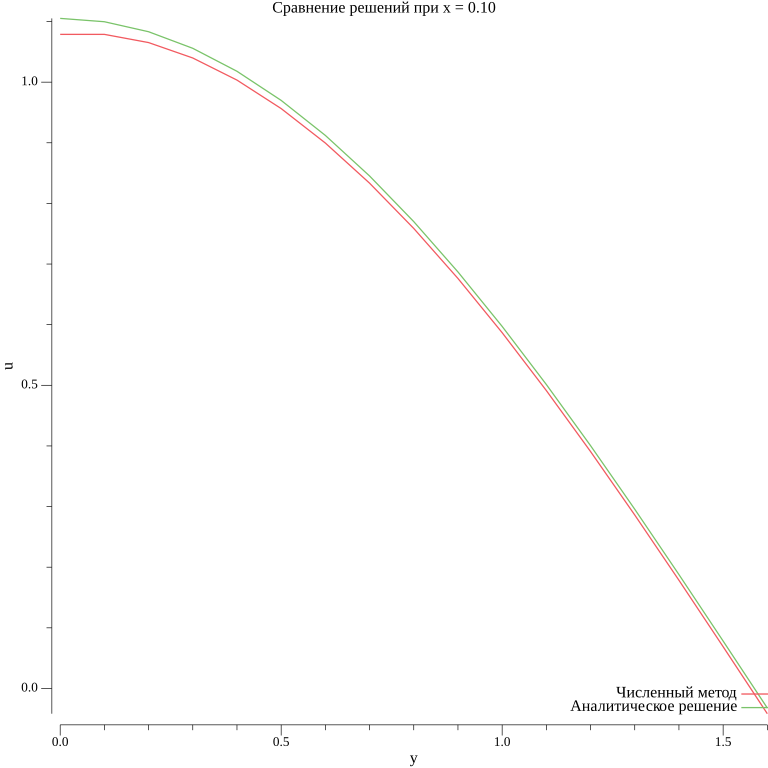
\includegraphics[scale=0.6]{1plot_x_0.10.png}
\\

\\
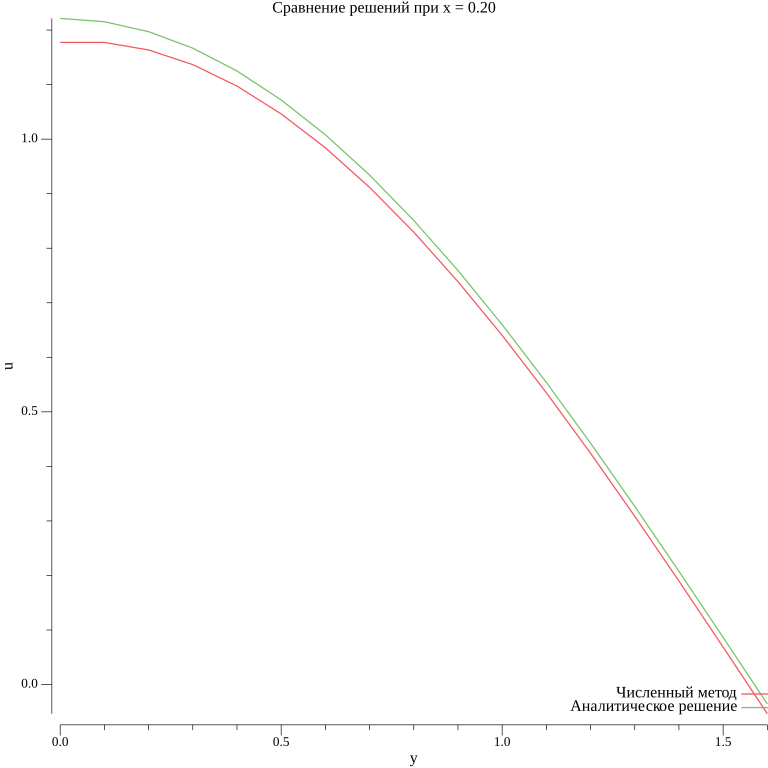
\includegraphics[scale=0.6]{1plot_x_0.20.png}
\\

\\
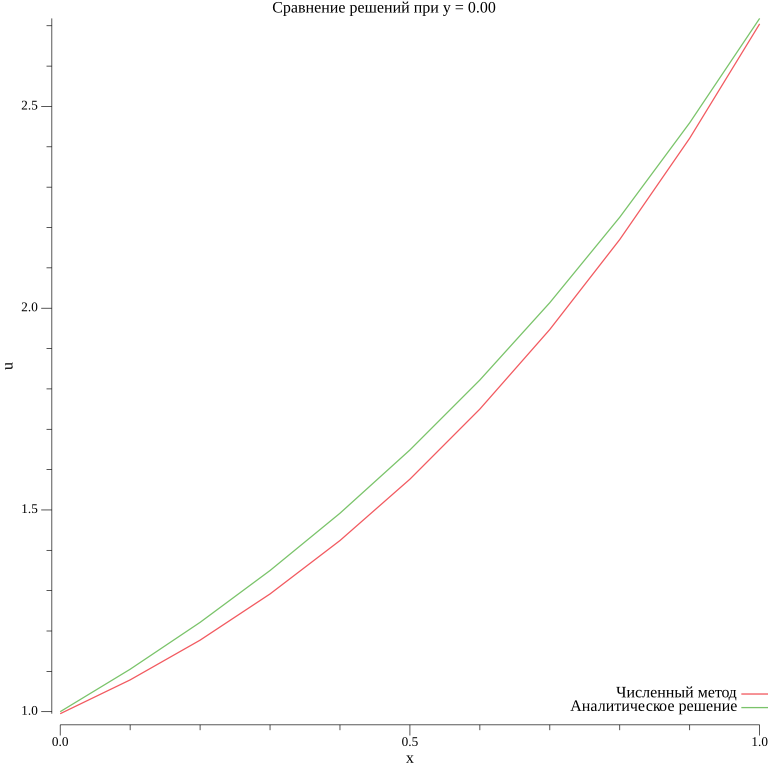
\includegraphics[scale=0.6]{1plot_y_0.00.png}
\\

\\
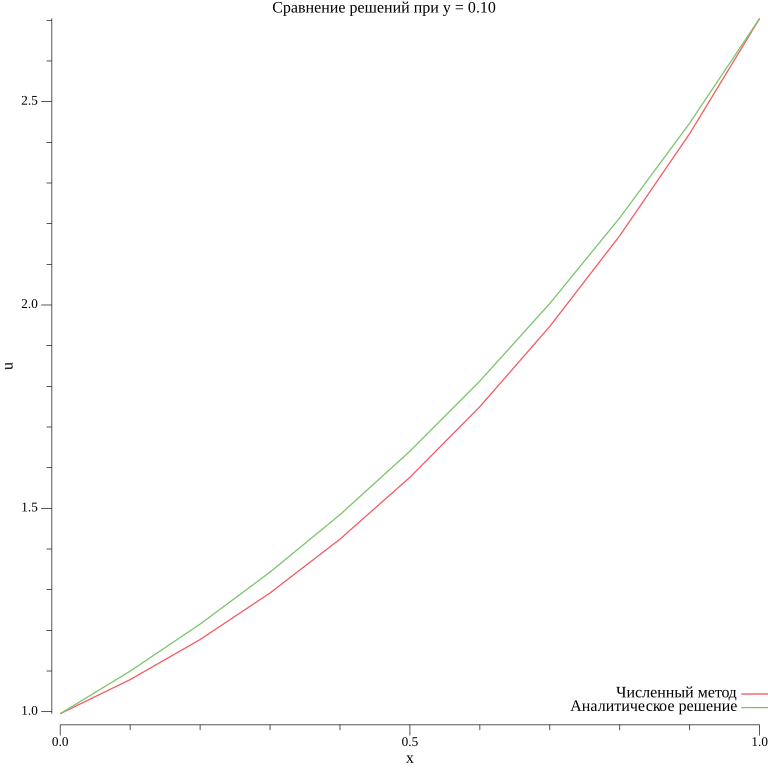
\includegraphics[scale=0.6]{1plot_y_0.10.png}
\\

\\
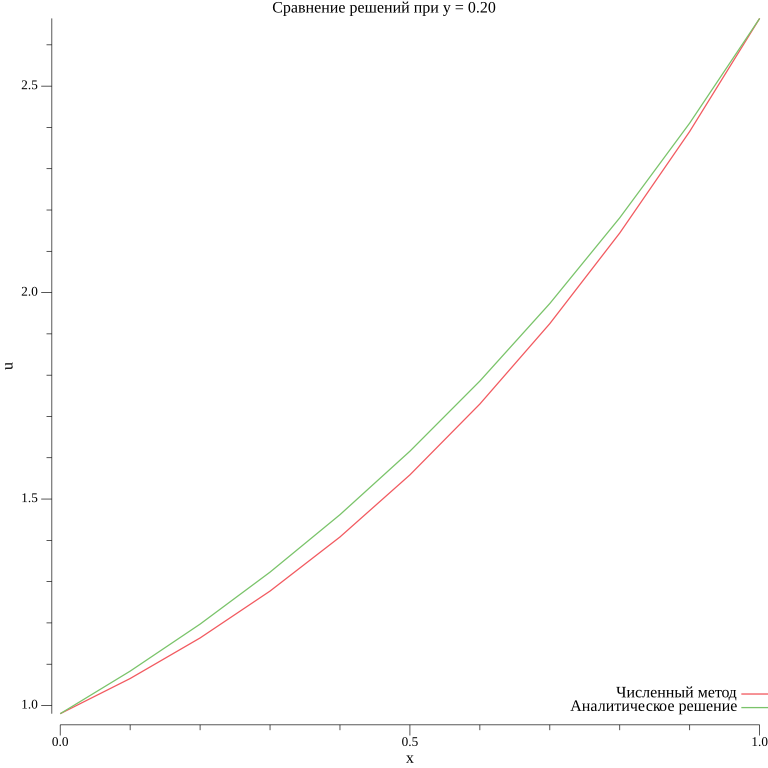
\includegraphics[scale=0.6]{1plot_y_0.20.png}
\\


\subsection*{Метод простых итераций с верхней релаксацией}
\\
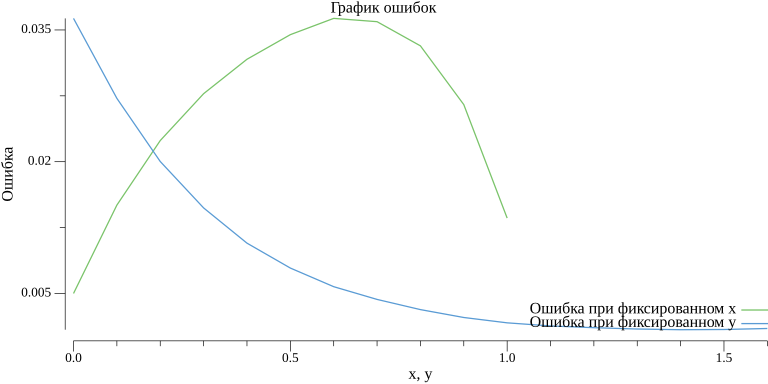
\includegraphics[scale=0.6]{error_plot_2.png}
\\

\\
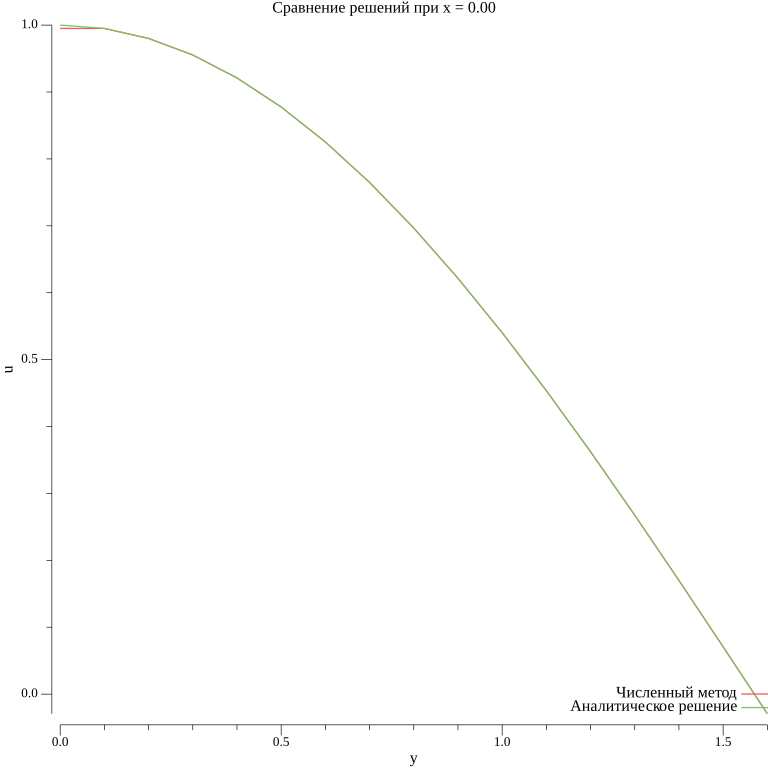
\includegraphics[scale=0.6]{2plot_x_0.00.png}
\\

\\
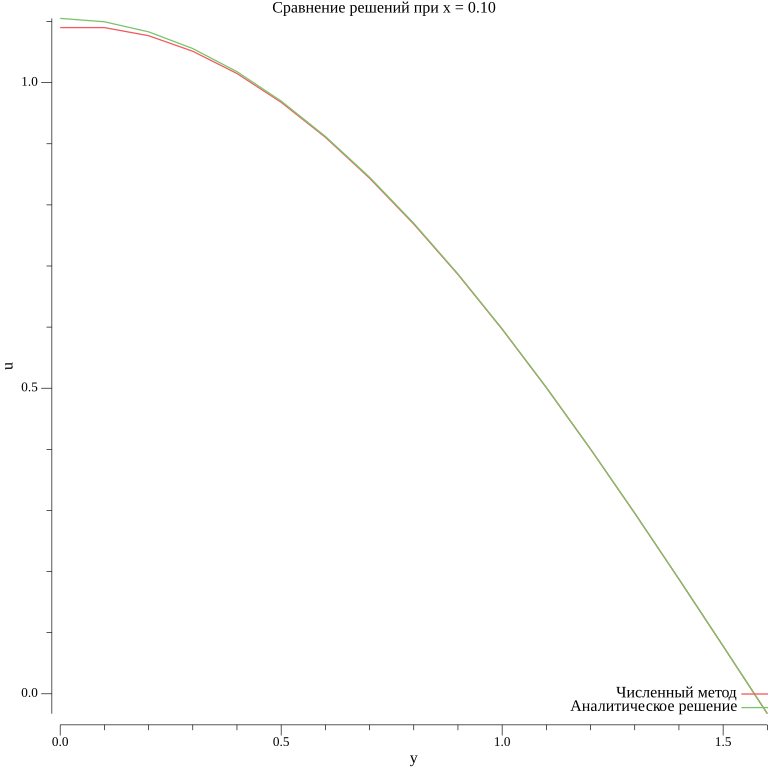
\includegraphics[scale=0.6]{2plot_x_0.10.png}
\\

\\
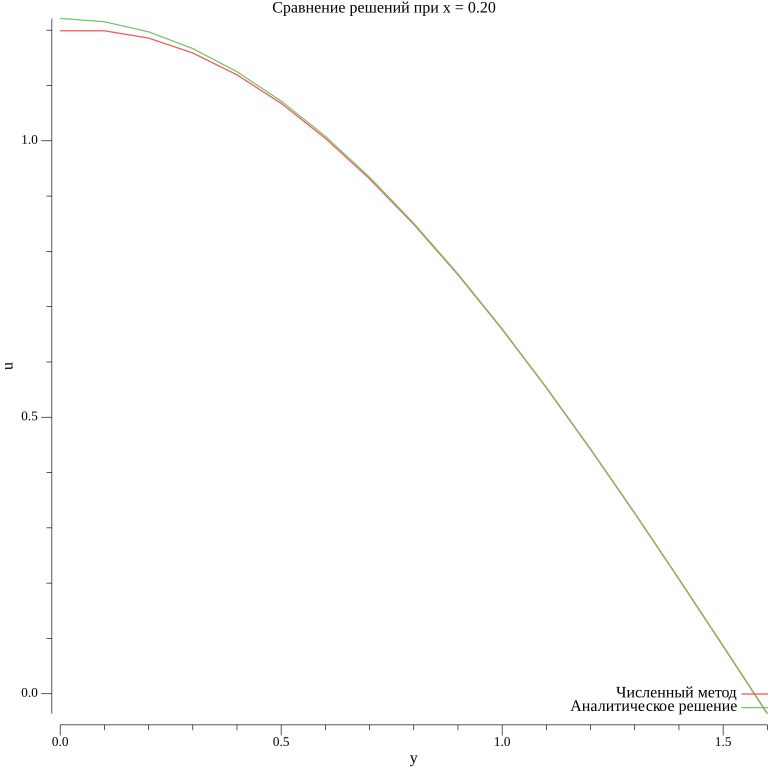
\includegraphics[scale=0.6]{2plot_x_0.20.png}
\\

\\
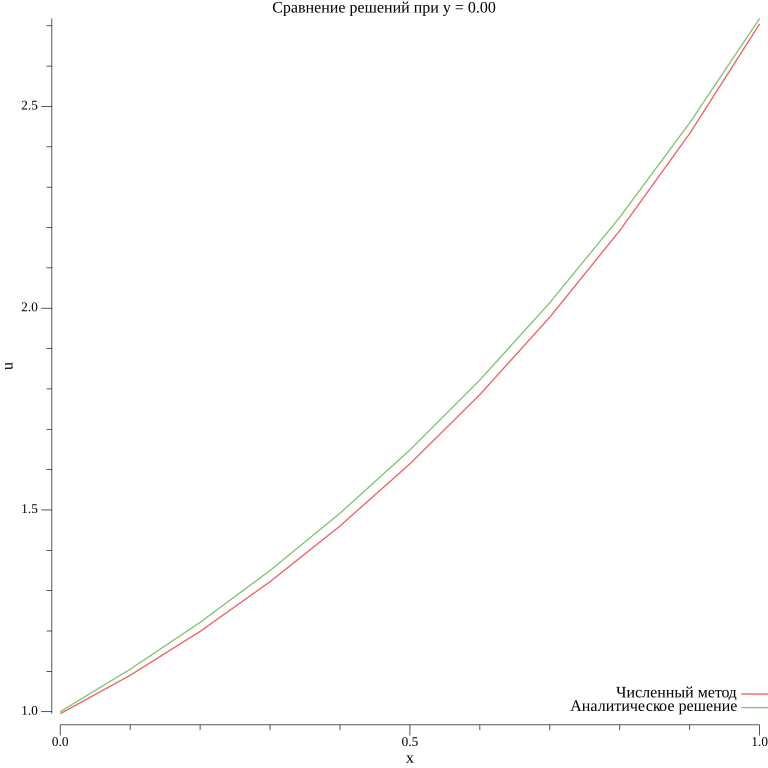
\includegraphics[scale=0.6]{2plot_y_0.00.png}
\\

\\
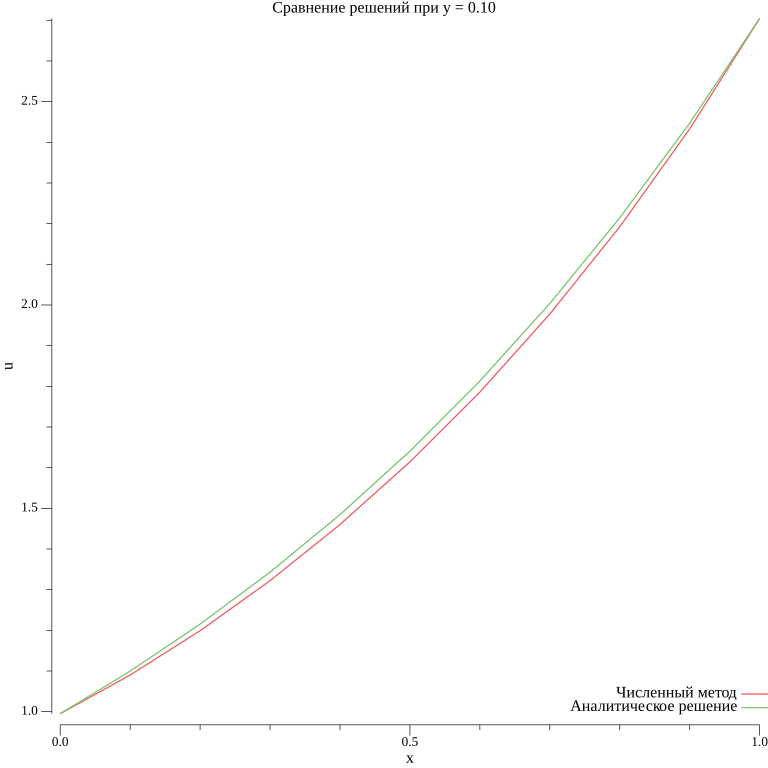
\includegraphics[scale=0.6]{2plot_y_0.10.png}
\\

\\
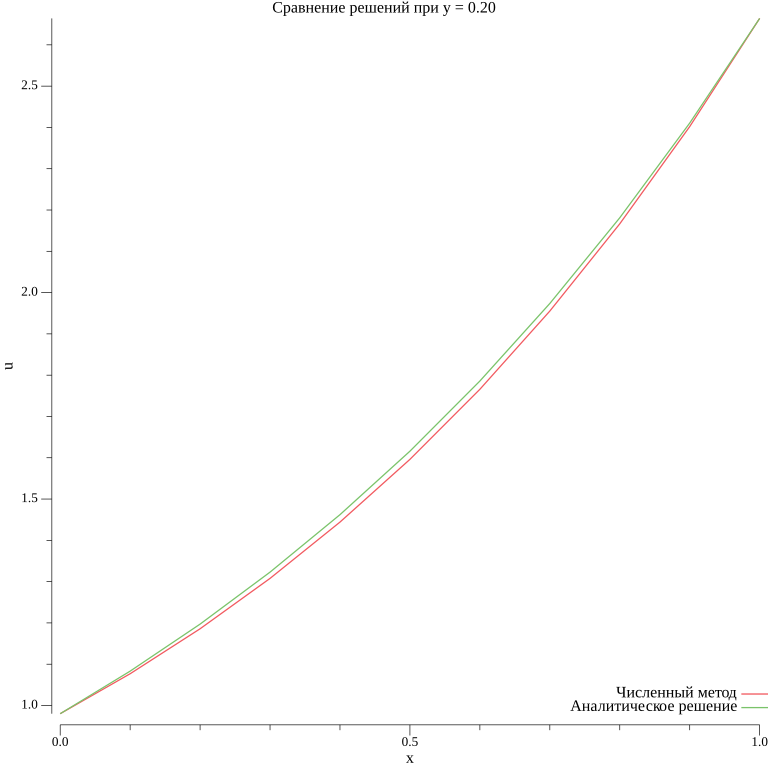
\includegraphics[scale=0.6]{2plot_y_0.20.png}
\\

\subsection*{Вывод}

В ходе выполнения лабораторной работы мной была успешно решена задача с начальными и граничными условиями для уравнения эллиптического типа. 
Я применил три разнообразных метода для решения соответствующих систем линейных алгебраических уравнений и осуществил анализ точности полученных результатов, 
сопоставив их с заданными параметрами точности.
\end{document}